% 图 62.1 —— 由 `checks/emit_hand.py` 自动拼出（probe 精测 + prims2 图元分解）
%%
% ⚠ 这是**稿子不是成品**：跑 `checks/checkhand.py 62.1` 看指标 + 看叠合图。
%%
%% ⚠ 待核：
%   · 本图 probe 报出阴影族 2 个 —— **本脚本不生成阴影**（要照原书手写）；prims2 的 strokes 里可能含阴影线，核对时留意别画重
%   · 可疑字形 2 项（空心圈 ⊙ 常被认成字母 o）—— 见文件末
%%
\documentclass[12pt]{standalone}
\usepackage{fontspec}
\setsansfont{Arial}
\newfontfamily\mfallback{DejaVu Sans}
\usepackage{tikz}
\begin{document}
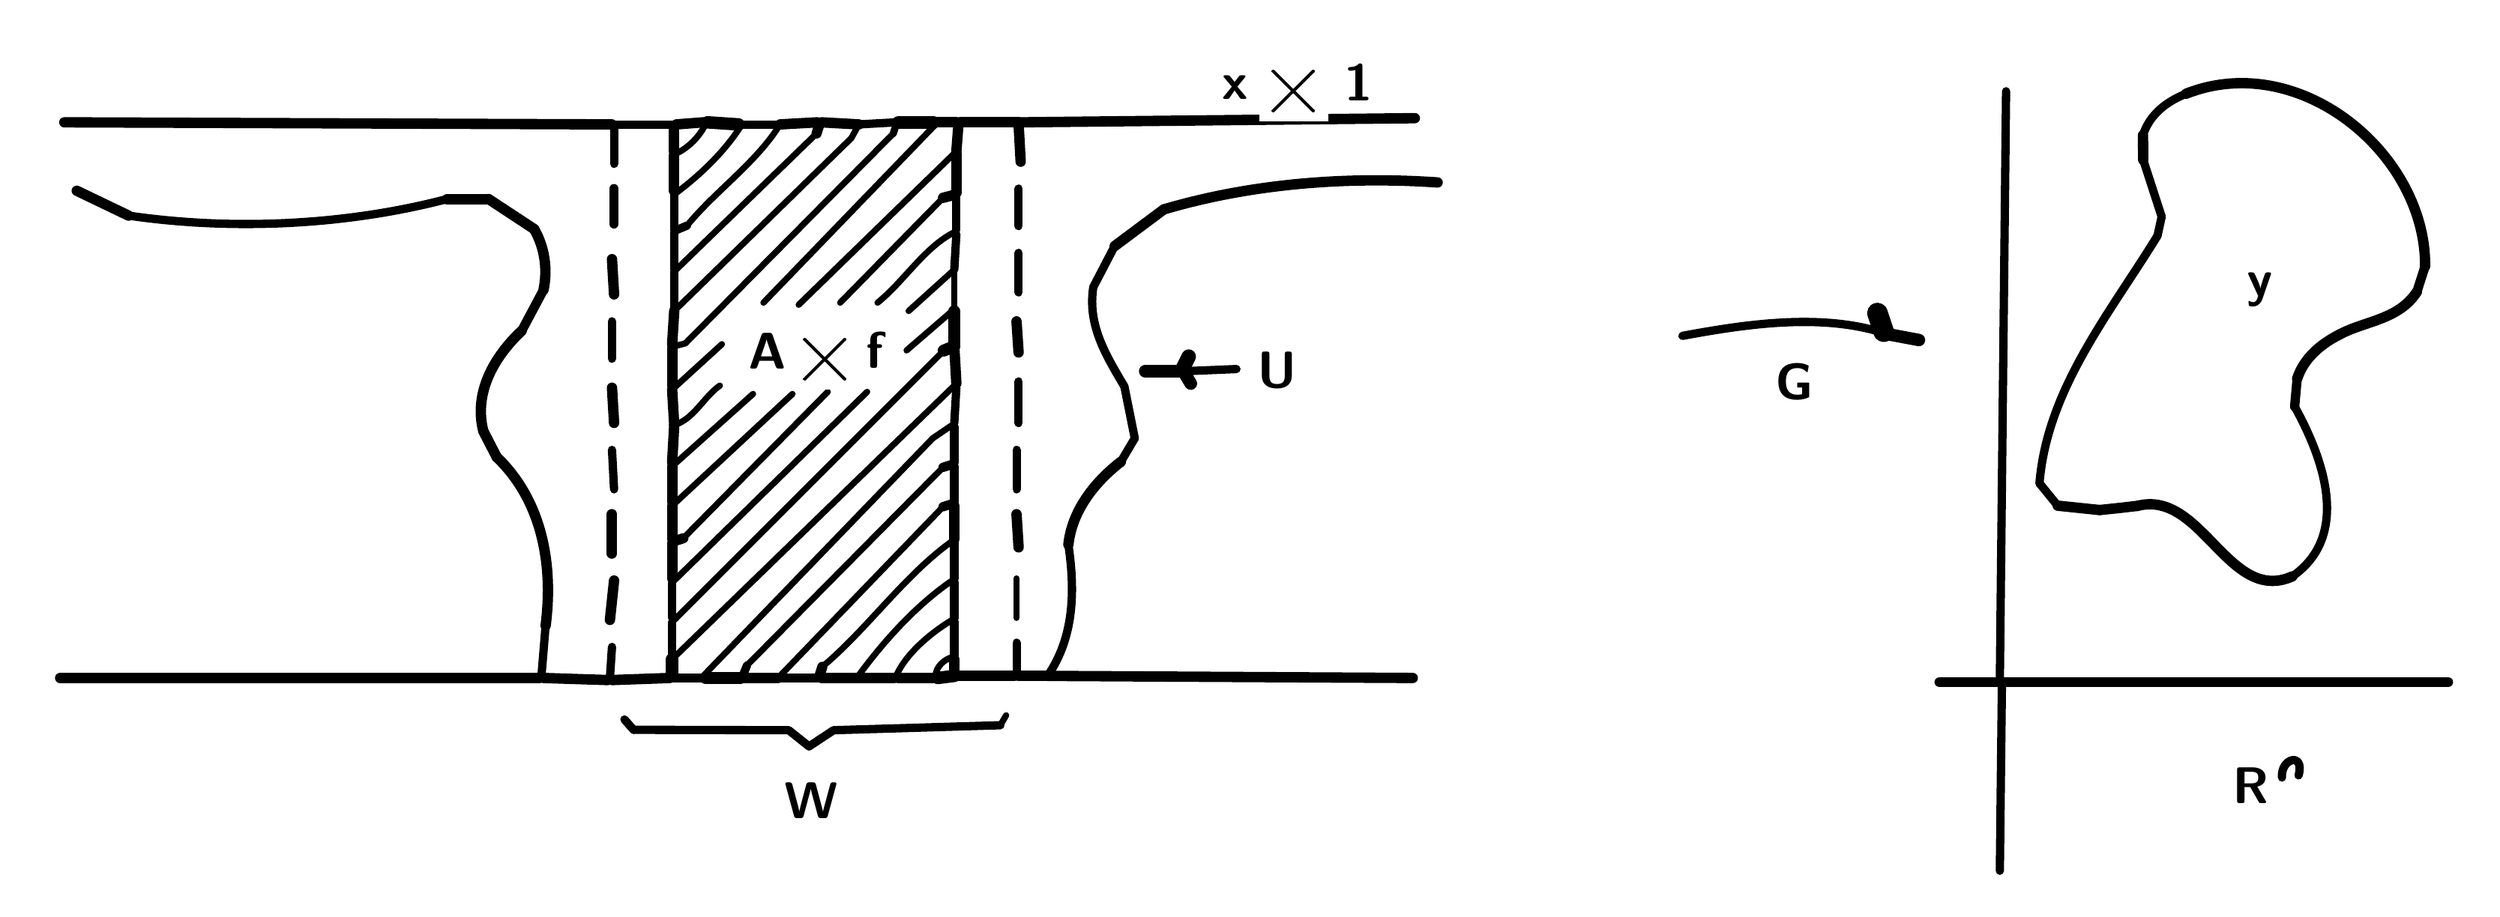
\begin{tikzpicture}[x=1pt, y=-1pt, line width=3.0pt, line cap=round, line join=round]

  %% ════ 直线段（prims2 的 strokes）════
  \draw[line width=3.0pt] (389.0,179.0) -- (319.4,249.6);
  \draw[line width=4.9pt] (319.4,249.6) -- (315.0,251.0);
  \draw[line width=5.0pt] (315.0,63.0) -- (315.0,51.0);
  \draw[line width=4.0pt] (451.0,101.0) -- (451.0,85.0);
  \draw[line width=3.0pt] (316.0,139.0) -- (400.4,56.6);
  \draw[line width=3.0pt] (400.4,56.6) -- (404.0,50.0);
  \draw[line width=5.0pt] (286.0,132.0) -- (285.0,115.0);
  \draw[line width=5.0pt] (453.0,49.0) -- (481.0,49.0);
  \draw[line width=5.0pt] (672.0,47.0) -- (482.0,49.0);
  \draw[line width=3.0pt] (315.0,157.0) -- (320.4,155.6);
  \draw[line width=3.0pt] (320.4,155.6) -- (420.6,54.4);
  \draw[line width=3.5pt] (420.6,54.4) -- (422.0,50.0);
  \draw[line width=5.0pt] (450.0,84.0) -- (444.6,85.4);
  \draw[line width=3.0pt] (444.6,85.4) -- (395.0,136.0);
  \draw[line width=5.0pt] (314.0,158.0) -- (314.0,176.0);
  \draw[line width=5.0pt] (314.0,213.0) -- (315.0,195.0);
  \draw[line width=4.0pt] (450.0,306.0) -- (450.0,290.0);
  \draw[line width=3.0pt] (315.0,289.0) -- (444.9,159.1);
  \draw[line width=5.8pt] (444.9,159.1) -- (450.0,157.0);
  \draw[line width=4.5pt] (286.0,81.0) -- (286.0,98.0);
  \draw[line width=5.0pt] (252.0,317.0) -- (283.0,318.0);
  \draw[line width=5.0pt] (314.0,252.0) -- (314.0,269.0);
  \draw[line width=4.0pt] (316.0,101.0) -- (321.2,98.8);
  \draw[line width=4.0pt] (480.0,315.0) -- (480.0,300.0);
  \draw[line width=9.9pt] (895.0,141.0) -- (898.0,150.0);
  \draw[line width=5.0pt] (1170.0,319.0) -- (956.0,319.0);
  \draw[line width=5.0pt] (450.0,308.0) -- (450.0,316.0);
  \draw[line width=4.0pt] (285.0,163.0) -- (285.0,145.0);
  \draw[line width=4.0pt] (315.0,84.0) -- (315.0,101.0);
  \draw[line width=4.0pt] (314.0,307.0) -- (314.0,290.0);
  \draw[line width=4.0pt] (481.0,131.0) -- (481.0,112.0);
  \draw[line width=5.0pt] (953.0,319.0) -- (925.0,319.0);
  \draw[line width=5.0pt] (451.0,175.0) -- (450.0,157.0);
  \draw[line width=4.0pt] (450.0,215.0) -- (450.0,232.0);
  \draw[line width=3.0pt] (427.0,159.0) -- (449.0,140.0);
  \draw[line width=7.0pt] (563.0,162.0) -- (560.0,168.0);
  \draw[line width=5.5pt] (450.0,140.0) -- (450.0,157.0);
  \draw[line width=5.0pt] (481.0,254.0) -- (480.0,238.0);
  \draw[line width=5.0pt] (285.0,50.0) -- (21.0,49.0);
  \draw[line width=5.0pt] (384.0,49.0) -- (366.0,50.0);
  \draw[line width=5.0pt] (329.0,49.0) -- (316.0,50.0);
  \draw[line width=3.0pt] (316.0,120.0) -- (383.6,54.4);
  \draw[line width=4.9pt] (383.6,54.4) -- (385.0,50.0);
  \draw[line width=3.0pt] (315.0,270.0) -- (408.0,179.0);
  \draw[line width=5.0pt] (286.0,194.0) -- (285.0,177.0);
  \draw[line width=4.0pt] (530.3,212.7) -- (537.0,201.4);
  \draw[line width=4.0pt] (537.0,201.4) -- (532.0,176.4);
  \draw[line width=4.0pt] (517.0,128.5) -- (527.3,108.7);
  \draw[line width=5.0pt] (527.3,108.7) -- (551.0,91.0);
  \draw[line width=5.0pt] (495.0,316.0) -- (481.0,316.0);
  \draw[line width=5.0pt] (495.0,316.0) -- (671.0,317.0);
  \draw[line width=6.0pt] (915.0,154.0) -- (899.0,151.0);
  \draw[line width=5.0pt] (315.0,140.0) -- (314.0,156.0);
  \draw[line width=4.9pt] (385.0,316.0) -- (386.4,311.6);
  \draw[line width=5.0pt] (285.0,318.0) -- (313.0,317.0);
  \draw[line width=4.5pt] (384.0,317.0) -- (367.0,317.0);
  \draw[line width=5.0pt] (450.0,234.0) -- (450.0,250.0);
  \draw[line width=5.0pt] (386.0,49.0) -- (404.0,50.0);
  \draw[line width=6.0pt] (331.0,49.0) -- (346.0,50.0);
  \draw[line width=4.0pt] (451.0,103.0) -- (450.0,120.0);
  \draw[line width=3.0pt] (315.0,177.0) -- (338.0,156.0);
  \draw[line width=4.0pt] (450.0,194.0) -- (451.0,177.0);
  \draw[line width=4.0pt] (314.0,288.0) -- (314.0,271.0);
  \draw[line width=4.0pt] (314.0,50.0) -- (286.0,50.0);
  \draw[line width=3.0pt] (372.0,180.0) -- (315.0,233.0);
  \draw[line width=4.0pt] (315.0,102.0) -- (315.0,120.0);
  \draw[line width=3.0pt] (450.0,64.0) -- (375.0,137.0);
  \draw[line width=5.0pt] (479.0,316.0) -- (450.0,316.0);
  \draw[line width=5.0pt] (423.0,317.0) -- (440.0,317.0);
  \draw[line width=4.0pt] (481.0,99.0) -- (481.0,81.0);
  \draw[line width=6.0pt] (314.0,316.0) -- (314.0,308.0);
  \draw[line width=4.0pt] (291.0,337.0) -- (295.4,342.0);
  \draw[line width=4.0pt] (295.4,342.0) -- (370.2,342.2);
  \draw[line width=4.0pt] (370.2,342.2) -- (380.0,350.0);
  \draw[line width=5.0pt] (386.0,317.0) -- (403.0,317.0);
  \draw[line width=4.5pt] (449.0,214.0) -- (444.6,215.4);
  \draw[line width=3.0pt] (444.6,215.4) -- (350.1,310.9);
  \draw[line width=4.0pt] (350.1,310.9) -- (348.0,316.0);
  \draw[line width=3.0pt] (450.0,176.0) -- (315.0,307.0);
  \draw[line width=5.0pt] (314.0,250.0) -- (314.0,234.0);
  \draw[line width=5.0pt] (481.0,50.0) -- (482.0,68.0);
  \draw[line width=5.0pt] (285.0,257.0) -- (285.0,238.0);
  \draw[line width=4.0pt] (450.0,213.0) -- (450.0,196.0);
  \draw[line width=4.5pt] (315.0,317.0) -- (328.0,317.0);
  \draw[line width=5.0pt] (480.0,145.0) -- (481.0,160.0);
  \draw[line width=3.0pt] (358.0,136.0) -- (441.0,50.0);
  \draw[line width=4.0pt] (315.0,121.0) -- (315.0,139.0);
  \draw[line width=4.0pt] (954.0,318.0) -- (957.0,34.0);
  \draw[line width=4.0pt] (286.0,69.0) -- (286.0,51.0);
  \draw[line width=3.0pt] (450.0,122.0) -- (450.0,139.0);
  \draw[line width=4.0pt] (954.0,410.0) -- (955.0,320.0);
  \draw[line width=4.5pt] (449.0,233.0) -- (444.6,234.4);
  \draw[line width=3.0pt] (444.6,234.4) -- (366.0,316.0);
  \draw[line width=5.0pt] (314.0,178.0) -- (315.0,195.0);
  \draw[line width=4.0pt] (481.0,174.0) -- (481.0,194.0);
  \draw[line width=3.0pt] (449.0,195.0) -- (439.6,201.4);
  \draw[line width=3.0pt] (439.6,201.4) -- (329.0,316.0);
  \draw[line width=4.0pt] (348.0,50.0) -- (366.0,50.0);
  \draw[line width=4.0pt] (285.0,302.0) -- (284.0,317.0);
  \draw[line width=4.0pt] (450.0,269.0) -- (450.0,252.0);
  \draw[line width=5.5pt] (347.0,317.0) -- (330.0,317.0);
  \draw[line width=5.0pt] (365.0,317.0) -- (348.0,317.0);
  \draw[line width=4.0pt] (422.0,49.0) -- (404.0,50.0);
  \draw[line width=3.0pt] (480.0,269.0) -- (480.0,288.0);
  \draw[line width=6.0pt] (542.0,169.0) -- (559.0,169.0);
  \draw[line width=4.0pt] (380.0,350.0) -- (391.8,342.2);
  \draw[line width=4.0pt] (391.8,342.2) -- (472.2,339.8);
  \draw[line width=3.0pt] (472.2,339.8) -- (475.0,335.0);
  \draw[line width=5.0pt] (284.0,289.0) -- (286.0,270.0);
  \draw[line width=4.0pt] (586.0,168.0) -- (562.0,169.0);
  \draw[line width=6.0pt] (440.0,49.0) -- (423.0,49.0);
  \draw[line width=4.0pt] (480.0,207.0) -- (480.0,226.0);
  \draw[line width=3.0pt] (353.0,180.0) -- (315.0,214.0);
  \draw[line width=4.0pt] (286.0,226.0) -- (285.0,207.0);
  \draw[line width=6.1pt] (564.0,175.0) -- (561.0,170.0);
  \draw[line width=5.0pt] (451.0,63.0) -- (452.0,50.0);
  \draw[line width=4.0pt] (450.0,288.0) -- (450.0,271.0);
  \draw[line width=3.0pt] (449.0,121.0) -- (428.0,140.0);
  \draw[line width=5.0pt] (442.0,49.0) -- (451.0,49.0);
  \draw[line width=5.0pt] (451.0,64.0) -- (451.0,83.0);
  \draw[line width=6.0pt] (442.0,317.0) -- (450.0,316.0);
  \draw[line width=5.0pt] (314.0,215.0) -- (314.0,232.0);
  \draw[line width=5.0pt] (315.0,82.0) -- (315.0,65.0);
  \draw[line width=5.0pt] (19.0,317.0) -- (250.0,317.0);
  \draw[line width=5.0pt] (403.0,317.0) -- (421.0,317.0);
  \draw[line width=5.0pt] (27.0,82.0) -- (52.0,94.0);
  \draw[line width=5.0pt] (205.5,86.0) -- (225.5,86.0);
  \draw[line width=5.0pt] (225.5,86.0) -- (247.5,100.5);
  \draw[line width=4.5pt] (252.0,129.8) -- (241.5,149.5);
  \draw[line width=5.0pt] (223.0,198.0) -- (229.4,210.4);
  \draw[line width=4.0pt] (253.0,291.8) -- (251.0,316.0);
  \draw[line width=4.5pt] (1096.1,186.1) -- (1097.3,172.7);
  \draw[line width=4.5pt] (1155.0,130.8) -- (1159.0,118.4);
  \draw[line width=5.0pt] (1023.0,55.2) -- (1023.1,67.1);
  \draw[line width=4.0pt] (1023.1,67.1) -- (1032.0,94.5);
  \draw[line width=4.0pt] (1032.0,94.5) -- (1030.0,103.7);
  \draw[line width=4.0pt] (973.1,223.1) -- (981.9,233.9);
  \draw[line width=5.0pt] (981.9,233.9) -- (1002.1,236.0);
  \draw[line width=5.0pt] (1002.1,236.0) -- (1011.7,235.0);
  \draw[line width=5.0pt] (1011.7,235.0) -- (1020.3,234.0);

  %% ════ 曲线（prims2 的 curves —— 三段式，坐标同为 (y,x)）════
  \draw[line width=4.0pt] (801.0,152.0) .. controls (831.0,146.4) and (866.4,141.2) .. (896.0,150.0);
  \draw[line width=3.0pt] (449.0,307.0) .. controls (445.2,307.9) and (441.0,311.8) .. (441.0,316.0);
  \draw[line width=3.0pt] (321.2,98.8) .. controls (334.4,82.5) and (354.7,68.4) .. (366.0,50.0);
  \draw[line width=3.0pt] (347.0,51.0) .. controls (339.1,63.3) and (327.5,74.4) .. (316.0,83.0);
  \draw[line width=3.0pt] (422.0,316.0) .. controls (426.7,305.2) and (438.7,295.2) .. (449.0,289.0);
  \draw[line width=4.0pt] (495.0,316.0) .. controls (507.8,297.3) and (508.3,275.1) .. (505.0,252.7);
  \draw[line width=5.0pt] (505.0,252.7) .. controls (506.7,236.6) and (517.3,222.8) .. (530.3,212.7);
  \draw[line width=4.0pt] (532.0,176.4) .. controls (523.4,161.8) and (514.1,147.1) .. (517.0,128.5);
  \draw[line width=5.0pt] (551.0,91.0) .. controls (592.3,78.8) and (637.9,74.9) .. (683.0,78.0);
  \draw[line width=3.0pt] (450.0,102.0) .. controls (435.6,109.3) and (425.6,125.9) .. (413.0,136.0);
  \draw[line width=3.0pt] (386.4,311.6) .. controls (408.5,293.0) and (425.8,267.6) .. (449.0,251.0);
  \draw[line width=3.0pt] (330.0,50.0) .. controls (327.4,55.7) and (321.7,61.4) .. (316.0,64.0);
  \draw[line width=3.0pt] (337.0,176.0) .. controls (329.3,181.3) and (324.5,192.2) .. (315.0,195.0);
  \draw[line width=4.0pt] (1098.0,364.0) .. controls (1101.1,352.6) and (1089.3,355.5) .. (1090.0,365.0);
  \draw[line width=3.0pt] (449.0,270.0) .. controls (431.8,281.7) and (415.6,299.6) .. (403.0,317.0);
  \draw[line width=4.0pt] (52.0,94.0) .. controls (102.6,101.4) and (157.4,98.6) .. (205.5,86.0);
  \draw[line width=5.0pt] (247.5,100.5) .. controls (252.5,109.3) and (254.1,119.6) .. (252.0,129.8);
  \draw[line width=5.0pt] (241.5,149.5) .. controls (228.2,162.0) and (218.2,179.4) .. (223.0,198.0);
  \draw[line width=5.0pt] (229.4,210.4) .. controls (251.4,231.5) and (256.8,262.3) .. (253.0,291.8);
  \draw[line width=4.0pt] (1095.0,268.0) .. controls (1123.7,248.1) and (1109.5,210.2) .. (1096.1,186.1);
  \draw[line width=5.0pt] (1097.3,172.7) .. controls (1100.5,162.8) and (1108.6,156.0) .. (1117.6,151.4);
  \draw[line width=5.0pt] (1117.6,151.4) .. controls (1130.3,144.6) and (1146.0,144.4) .. (1155.0,130.8);
  \draw[line width=5.0pt] (1159.0,118.4) .. controls (1159.3,63.9) and (1098.3,13.7) .. (1043.8,35.2);
  \draw[line width=4.0pt] (1043.8,35.2) .. controls (1034.3,39.0) and (1026.2,45.2) .. (1023.0,55.2);
  \draw[line width=4.0pt] (1030.0,103.7) .. controls (1006.7,141.6) and (976.8,177.7) .. (973.1,223.1);
  \draw[line width=5.0pt] (1020.3,234.0) .. controls (1051.4,226.0) and (1064.2,281.7) .. (1095.0,268.0);

  %% ════ 标签（probe 直接给的 \node 行）════
  %% ⚠ 全部补了 fill=white：文字在最上层，否则与曲线交叉干扰
     \node[anchor=center,inner sep=0pt,fill=white,font=\fontsize{38.0}{47.5}\selectfont] at (585.3,32.0) {\textsf{\textbf{\textit{x}}}};   % box(574,18,20,23)
     \node[anchor=center,inner sep=0pt,fill=white,font=\fontsize{28.9}{36.1}\selectfont] at (644.9,30.0) {\textsf{\textbf{1}}};   % box(637,19,9,21)
     \node[anchor=center,inner sep=0pt,fill=white,font=\fontsize{36.0}{45.0}\selectfont] at (613.6,34.2) {\textsf{\textbf{×}}};   % box(605,23,16,17)
     \node[anchor=center,inner sep=0pt,fill=white,font=\fontsize{29.2}{36.4}\selectfont] at (1079.7,129.7) {\textsf{\textbf{\textit{y}}}};   % box(1071,117,17,22)
     \node[anchor=center,inner sep=0pt,fill=white,font=\fontsize{27.8}{34.7}\selectfont] at (412.5,159.0) {\textsf{\textbf{\textit{f}}}};   % box(407,147,10,23)
     \node[anchor=center,inner sep=0pt,fill=white,font=\fontsize{30.3}{37.9}\selectfont] at (359.8,159.5) {\textsf{\textbf{\textit{A}}}};   % box(347,148,20,22)
     \node[anchor=center,inner sep=0pt,fill=white,font=\fontsize{34.9}{43.6}\selectfont] at (387.6,163.6) {\textsf{\textbf{×}}};   % box(379,153,16,16)
     \node[anchor=center,inner sep=0pt,fill=white,font=\fontsize{30.4}{38.0}\selectfont] at (605.5,168.3) {\textsf{\textbf{\textit{U}}}};   % box(595,156,21,22)
     \node[anchor=center,inner sep=0pt,fill=white,font=\fontsize{29.9}{37.4}\selectfont] at (854.8,174.2) {\textsf{\textbf{\textit{G}}}};   % box(845,162,20,23)
     \node[anchor=center,inner sep=0pt,fill=white,font=\fontsize{30.0}{37.5}\selectfont] at (1075.0,369.0) {\textsf{\textbf{\textit{R}}}};   % box(1065,357,20,22)
     \node[anchor=center,inner sep=0pt,fill=white,font=\fontsize{29.2}{36.6}\selectfont] at (381.2,376.0) {\textsf{\textbf{\textit{W}}}};   % box(368,364,26,22)

  % 钉死画布：否则超出的图元/控制点会把页面撑大，1:1 回比就失准
  \pgfresetboundingbox
  \path[use as bounding box] (0,0) rectangle (1185,422);
\end{tikzpicture}
\end{document}

% ⚠ 待核清单（probe 拿不准，人眼过一遍）：
%   · 未识别/跳过：⑤ 跳过/未识别的字形
%   · 未识别/跳过：box(542,162,47,15)
